\documentclass{article}
% pre\'ambulo

\usepackage{lmodern}
\usepackage[T1]{fontenc}
\usepackage{graphicx}
\usepackage[spanish,activeacute]{babel}
\usepackage{mathtools}

\title{Agujeros negros primordiales como modelo de Materia oscura.}
\author{Luis A. Escamilla, Jonathan Rinc\'on}



\begin{document}
\maketitle
% cuerpo del documento

  \begin{@twocolumnfalse}
    \maketitle
    \begin{abstract}
      Los agujeros negros son regiones en el espacio-tiempo que generan un campo gravitatorio tal que ninguna part\'icula material, ni siquiera la luz, puede escapar. Sin embargo, con base en las observaciones se han podido determinar algunas propiedades fundamentales como: la posici\'on, su masa, y recientemente [11 de febrero de 2016] la colaboraci\'on LIGO detect\'o por primera vez ondas gravitacionales debido al choque de dos agujeros negros.
Aunque la formaci\'on de agujeros negros se relaciona habitualmente con el colapso gravitacional de una estrella lo suficientemente masiva, en los primeros instantes del Big Bang, de acuerdo con el modelo est\'andar de part\'iculas, hubo regiones donde la densidad era tan grande que pudieron haberse formado agujeros negros primordiales (PBHs) debido al colapso gravitacional. En este trabajo, de acuerdo con la premisa de la existencia de dichos agujeros negros primordiales, se har\'a un breve repaso a su historia, las teor\'ias y modelos sobre estos fen\'omenos y c\'omo se han propuesto como candidatos a ser materia oscura.
    \end{abstract}
  \end{@twocolumnfalse}



\section*{Big bang} 
\subsection*{Recuento hist\'orico}
Para poder comenzar a hablar sobre los hoyos negros primordiales debemos hacer un breve repaso a lo que se denomina teor\'ia del Big Bang. Este modelo cosmol\'ogico afirma que nuestro Universo provino de una singularidad en la que toda la materia, energ\'ia e incluso el espacio-tiempo estaban confinados en un punto incre\'iblemente denso y caliente, que luego pas\'o a expandirse de manera acelerada, enfri\'andose poco a poco y formando la materia que hoy conocemos. 

Podr\'iamos decir que la teor\'ia del Big Bang empez\'o con la teor\'ia General de la Relatividad de Einstein publicada en 1915, cuya base es que la deformaci\'on del espacio-tiempo provocada por objetos masivos provoca lo que nosotros conocemos como gravedad. 

Pese a los esfuerzos de Einstein de crear un universo est\'atico, Alexander Friedmann y Georges Lemaitre encontraron soluciones (cada uno por su cuenta) de la teor\'ia de general que indicaban que el universo se expande. Y en 1931 Georges Lemaitre propuso que el universo provino de un ``\'atomo primigenio'' un punto en el que todo el universo converg\'ia, esta teor\'ia se sustentaba de las soluciones obtenidas de la relatividad general. Su l\'ogica es simple, debido a que el universo est\'a en expansi\'on si regres\'aramos en el tiempo, por ejemplo; 1 minuto el tama\~no del universo ser\'ia m\'as peque\~no que el de ahora, entonces que pasar\'ia si volvi\'eramos en el tiempo hasta $t=0$, entonces toda lo que conforma el universo estar\'ia en un s\'olo punto. A esto se le denomin\'o luego Big Bang. A\'un y cuando muchos autores se\~nalan que el motivo por el cual Lemaitre propuso esta teor\'ia, en que el universo fue ``creado'' o por lo menos no ha existido desde siempre como otras teor\'ias se\~nalaban (lo cual estaba de acuerdo con la doctrina cat\'olica), era por sus profundas ra\'ices religiosas, debido a que era un sacerdote. Sin embargo, esta idea ha permanecido hasta nuestros d\'ias.

Debemos enfatizar que esta exc\'entrica propuesta pudo haber estado basada adem\'as en las observaciones presentadas por Vesto Slipher y Carl Wilhelm sobre el corrimiento hacia el rojo en 11 galaxias que se alejaban de la Tierra en 1914 y de las observaciones realizadas por Edwin Hubble sobre las velocidades radiales de algunas nebulosas con respecto a la Tierra en 1929, que luego dar\'ian paso a la famosa ``ley de Hubble''.

Pero quiz\'as la mayor prueba del modelo del Big Bang fue el descubrimiento de la radiaci\'on de fondo de microondas o CMB (cosmic microwave background radiation) en 1965 realizada por Arno Penzias y Robert Wilson en los laboratorios Bell.  Cuya radiaci\'on correspond\'ia al de un cuerpo negro casi perfecto, con un pico de $\lambda=1.9 mm$ y una temperatura aproximada de $T=2.725 K$ [7].


\subsection*{Modelo del Big Bang caliente}
Este modelo es el m\'as aceptado, seg\'un el cual todo el universo era una bola de fuego primordial con una temperatura y presi\'on incre\'iblemente grande, que despu\'es de un cierto instante se expandi\'o, lo que llevo consecuentemente a enfriarse y crear los elementos que actualmente podemos estudiar.

Una pregunta muy frecuente sobre el Big Bang es su origen o lo que hab\'ia antes de que se produjera tal evento. Aunque esta pregunta es muy intrigante cualquier predicci\'on o teor\'ia que se\~nale alg\'un proceso antes del Big Bang es totalmente especulativa ya que se cree que en sus primeros momentos todas las fuerzas fundamentales (gravedad, electromagn\'etica, fuerza nuclear d\'ebil y fuerte) estaban unidas y hasta no tener una teor\'ia que pueda unificarlas no podemos explicar los procesos que ocurrieron.

 Aunque el hecho de preguntarse el origen del Big Bang suena algo muy normal esto podr\'ia ser un error, ya que preguntarse el ``antes'' del Big Bang no tiene sentido porque en ese punto super caliente y denso estaba incluso el espacio-tiempo. El tiempo mismo se cre\'o a partir del Big Bang.
 
Aun as\'i, el modelo est\'andar de part\'iculas elementales ha podido explicar los primeros instantes del Big Bang (despu\'es del primer segundo) y la evoluci\'on del universo una vez que \'este se enfri\'o para dar paso a la formaci\'on de los primeros elementos. Por lo que en esta secci\'on haremos un peque\~no repaso a dichas fases o etapas para comprender un poco m\'as sobre nuestro tema principal, la formaci\'on de los agujeros negros primordiales.

\subsection*{Primeros instantes despu\'es del Big Bang}
Se cree que los primeros instantes despu\'es del fen\'omeno cosmol\'ogico que di\'o paso al origen del universo, las 4 fuerzas fundamentales: la Gravedad, el Electromagnetismo, La fuerza nuclear Fuerte y D\'ebil. Estaban juntas en una \'unica fuerza fundamental que luego de un brev\'isimo periodo de tiempo ($10^{-42}$  a $10^{-36}$ segundos aproximadamente) empiezan a separarse una a una, por un mecanismo denominado ``ruptura de simetr\'ia''. 

\subsection*{Inflaci\'on}
Antes de ver cada una de las transiciones de fase ocurridas en el Big Bang debemos detenernos un momento en un proceso sumamente importante denominado ``inflaci\'on c\'osmica''. Esta teor\'ia introducida por primera vez en 1981 por Alan Guth, nos dice que hubo una \'epoca en el universo en que el factor de escala se aceler\'o r\'apidamente en s\'olo una fracci\'on de segundo. Es decir, el universo se expandi\'o de tal manera que en un periodo de tiempo aproximadamente de $10^{-36}-10^{-33}$ segundos) donde el universo creci\'o hasta llegar a tener un tama\~{n}o de $e^{60}$ veces el inicial.

Debido a este extraordinario proceso el universo pudo enfriarse r\'apidamente lo que di\'o paso a las etapas que discutiremos a continuaci\'on.

\textbf{Transici\'on GUT:} con una temperatura cercana a los $10^{16} GeV$, en este momento no hay distinci\'on entre la fuerza fuerte, d\'ebil y la electromagn\'etica. Estaban unidas en una \'unica fuerza y s\'olo la gravedad se separ\'o.
\begin{equation}
G \rightarrow SU(3) \otimes SU(2) \otimes U(1)
\end{equation}

\textbf{Transici\'on Electrod\'ebil:} con una temperatura cerca de los 100 GeV, la condensaci\'on de Higgs estaba ausente y los bosones $W^{-},Z^{-}$ tienen masa cero, con la ruptura de simetr\'ia electrod\'ebil ocurre la condensaci\'on de Higgs y obtenemos bosones  $W^{-}$  y  $Z^{-}$ masivos. 
\begin{equation}
SU(3) \otimes SU(2) \otimes U(1) \rightarrow SU(2) \otimes U(1)
\end{equation}
En esta transici\'on la tambi\'en fuerza electrod\'ebil se separa en la fuerza electromagn\'etica y la fuerza nuclear d\'ebil.

\textbf{Transici\'on de la materia quark-gluon a materia hadr\'onica:} con una temperatura de aproximadamente 200 MeV, el plasma de quarks-gluon se enfr\'ia hasta formar los hadrones, part\'iculas formadas por la uni\'on de quarks mediante la fuerza nuclear fuerte. 

\subsection*{Nucleos\'intesis}
Podr\'iamos hablar sobre las distintas etapas especulativas como la Era de Planck que se cree que tuvo lugar $10^{-42}$ segundos despu\'es del Big Bang y donde la temperatura era superior a los 100 MeV y muchas otras etapas m\'as, pero lo cierto es que el modelo del Big Bang caliente solo puede explicar efectivamente cuando el universo (debido a la expansi\'on c\'osmica) redujo la energ\'ia cin\'etica de las part\'iculas para poder formar n\'ucleos. A esta etapa se le llama nucleos\'intesis en la cual se crearon los primeros elementos cuando la temperatura era alrededor de $T=0.1 MeV$, 1 segundo despu\'es del Big Bang.

\subsection*{Dominaci\'on de la materia}
En los primeros momentos del Big Bang como sabemos la radiaci\'on era la que dominaba sobre la materia ya que debido a la gran temperatura del universo la energ\'ia cin\'etica de las part\'iculas no permit\'ia que \'estas pudieran unirse para formar n\'ucleos, por ende, la mayor parte de la energ\'ia del universo se encontraba en forma de radiaci\'on, pero debido a la expansi\'on del universo provoc\'o que \'este se enfriara y pudieran formarse los primeros n\'ucleos. Aproximadamente 70,000 a\~nos despu\'es del Big Bang las densidades de materia (no-relativista) conformados por los n\'ucleos at\'omicos y la radiaci\'on conformada por fotones fueron iguales. Esta transici\'on es muy importante desde el punto de vista del crecimiento de las perturbaciones de densidad como veremos m\'as adelante.

\subsection*{Recombinaci\'on}
Luego de aproximadamente 300,000 a\~nos del Big Bang, la densidad del universo disminuye y se forman los primeros \'atomos de hidr\'ogeno y helio, tambi\'en la radiaci\'on se desacopla de la materia hasta que puede viajar libremente. La imagen del CMB corresponde a estos fotones.
Luego de esto, millones de a\~nos despu\'es se formaron las primeras estrellas, las galaxias y los c\'umulos de galaxias por medio de procesos gravitatorios.

Como hemos visto el Big Bang es un fen\'omeno el cual conlleva una serie de procesos los cuales con el paso del tiempo dieron forma a lo que hoy conocemos como universo. Sin embargo, en los primeros momentos del universo cuando \'este todav\'ia era muy caliente y denso, pudo haber fluctuaciones en la densidad de materia del universo temprano las cuales pudieron haber originado regiones con mucha densidad hasta colapsar gravitacionalmente, a esto se conoce como ``agujero negro primordial''. Esta interesante idea surgi\'o por primera vez de Zel' Dovich y Novik en 1966. 


\section*{Materia Oscura} 
La idea de que debe haber materia invisible en el universo est\'a presente desde el a\~no 1933, cuando Fritz Zwicky realiz\'o observaciones sobre cuerpos astron\'omicos orbitando en la galaxia, de esta forma calcular la velocidad radial de la misma. Estas mediciones las realiz\'o sobre 8 galaxias del C\'umulo de Coma y se di\'o cuenta de que las velocidades radiales eran bastante grandes si se toma en cuenta \'unicamente la materia visible, para que las mediciones de las velocidades concordaran con el valor te\'orico el C\'umulo deb\'ia tener 400 veces m\'as masa de la que se observaba. Esta idea de Zwicky se dej\'o como un problema sin resolver, hasta que, 3 a\~nos despu\'es, Sinclair Smith realiz\'o observaciones similares en el C\'umulo de Virgo y lleg\'o a las mismas conclusiones de Zwicky. Esto ciment\'o la base de la idea sobre la existencia de materia invisible que es m\'as densa que la visible.

Para el a\~no 1975 ya estaba difundida la idea de que exist\'ia una gran cantidad de materia invisible en las galaxias, aunque no se supiera de d\'onde proven\'ia. El concepto de materia oscura surgi\'o de estas observaciones, pues la idea popular era que la materia faltante deb\'ia ser un nuevo tipo de materia, la cu\'al es no-bari\'onica e interact\'ua muy d\'ebilmente con la materia convencional.

\subsubsection*{Lente gravitacional}
Una de las evidencias acerca de la existencia de materia oscura proviene de las observaciones realizadas usando lentes gravitacionales.

 De acuerdo a la relatividad general, si la luz pasa cerca de un objeto muy masivo, la trayectoria de la luz se ver\'a curvada debido a la curvatura del espacio-tiempo provocada por el objeto masivo.  Las observaciones realizadas con lentes gravitacionales consisten en utilizar este fen\'omeno conocido como ``curvatura de la luz'' para poder determinar la cantidad de materia que se encuentra en un lugar. Existen 3 tipos de fen\'omenos de lente gravitacional: fuerte, d\'ebil y microlente. 
 
 \textbf{Fuerte:} aqu\'i se observan distorsiones muy claras y se puede llegar a apreciar la formaci\'on de figuras como arcos o anillos de Einstein.

 \textbf{D\'ebil:} en este fen\'omeno ocurren distorsiones d\'ebiles pero apreciables, pero debido a que son distorsiones d\'ebiles deben realizarse muchas mediciones para que se pueda asegurar que el fen\'omeno en cuesti\'on est\'a ocurriendo.

 \textbf{Microlente:} en este fen\'omeno no ocurre distorsi\'on aparente, pero si hay un cambio en la cantidad de luz recibida. Este es el fen\'omeno m\'as utilizado para intentar detectar materia oscura compacta.



\subsubsection*{Halo de Materia Oscura}
Se infiere que la materia oscura de una galaxia se encuentra en un halo casi esf\'erico alrededor de la misma. Estos halos no pueden ser observados directamente ya que est\'an hechos de materia oscura, pero se puede inferir su existencia debido a observaciones sobre el movimiento de estrellas y gas en las galaxias.

Si no existiesen los halos esf\'ericos, la velocidad rotacional de la galaxia disminuir\'ia a distancias grandes del centro de la galaxia, pero se ha observado que la velocidad de rotaci\'on de las galaxias no disminuye lejos del centro (Bosma, A., 1978, Universidad de Groningen), esto implica una de dos cosas, o que existe materia extra invisible alrededor de las galaxias para compensar este movimiento, o que la Relatividad General est\'a incompleta.

\subsubsection*{Candidatos a Materia Oscura}
A pesar de que se cuenta con una gran cantidad de observaciones que sirven como evidencia para demostrar la existencia de la materia oscura, a\'un no se sabe de qu\'e est\'a hecha. En general se proponen dos posibilidades: que exista una part\'icula de materia oscura o que sea alg\'un objeto compacto astrof\'isico  que no interact\'ue con la luz.

Un candidato a materia oscura es el neutrino, formando un tipo de materia oscura conocida como ``materia oscura caliente''. Esto quiere decir que las part\'iculas tienen velocidades relativistas en alg\'un momento. Otro candidato un poco mejor es un neutrino m\'as pesado (con una masa parecida a la de un prot\'on). Debido a su gran masa tendr\'a velocidades mucho menores a las del l\'imite relativista. A este tipo de materia se le conoce como ``materia oscura fr\'ia''. Tambi\'en est\'an los llamados ``part\'icula m\'as ligera supersim\'etrica'' (LSP) y las ``part\'iculas masivas d\'ebilmente interactuantes'' (WIMPs), que consisten en dos tipos hipot\'eticos de part\'iculas.

Se mencion\'o que tambi\'en hay objetos compactos astrof\'isicos que se cree podr\'ian ser materia oscura, \'estos objetos son los agujeros negros primordiales (PBHs) y los objetos masivos de halo compacto (MACHOs). Los MACHOs pueden ser tanto agujeros negros como estrellas de neutrones, o hasta enanas caf\'es, es el nombre que se le d\'a a un objeto compuesto de materia bari\'onica y que no emite (o emite muy poca) radiaci\'on. Los MACHOs han sido detectados con lentes gravitacionales usando el fen\'omeno de microlente aunque a\'un no se sabe con seguridad qu\'e son. Por \'ultimo est\'an los PBHs, de los cu\'ales se hablar\'a con m\'as detalle en secciones posteriores.

\subsubsection*{Modelo Lambda-CDM y par\'ametros de densidad}
El modelo $\Lambda$CDM es una parametrizaci\'on del modelo cosmol\'ogio del Big Bang, en donde se considera una constante cosmol\'ogica $\Lambda$ cuyo valor est\'a asociado con la energ\'ia oscura y la materia oscura fr\'ia (CDM).

Se le llama par\'ametro de densidad ($Omega$) a la raz\'on entre la densidad de energ\'ia y materia en el universo con la densidad cr\'itica, siendo esta \'ultima la densidad en la cual el universo deja de expandirse tras un tiempo infinito. Entonces este par\'ametro est\'a dado por

\begin{equation}
\Omega=\frac{\rho}{\rho_c}
\end{equation} 

siendo $\rho$ la densidad actual y $\rho_c$ la densidad cr\'itica, que est\'a dada por 

\begin{equation}
\rho_c(t)=\frac{3H^2}{8\pi G}
\end{equation}

donde H es el par\'ametro de Hubble. Si usamos estos valores en la ecuaci\'on de Friedmann 

\begin{equation}
H^2=\frac{8\pi G\rho}{3}-\frac{k}{a^2}
\end{equation}

obtenemos

\begin{equation}
\Omega -1=\frac{k}{a^2 H^2}=\Omega_k
\end{equation}

donde $k/a^2$ es la curvatura espacial del universo. A $\Omega_k$ se le considera como un par\'ametro de densidad relacionado con la curvatura del espacio. En el caso en que $k=0$ tenemos un universo plano, lo que implicar\'ia $\Omega_k=0$, y este caso es de mucho inter\'es pues el valor de $\Omega_k$, seg\'un observaciones, es $\Omega_k<0.005$

El modelo $\Lambda$CDM tambi\'en propone que $\Omega$ est\'a formado por varias componentes, y como $\Omega_k \approx 0$ entonces $\Omega \approx 1$, lo que nos da

\begin{equation}
\Omega=\Omega_b + \Omega_{DM} + \Omega_\Lambda \approx 1
\end{equation}

siendo $\Omega_b$ el par\'ametro de densidad de materia bari\'onica, $\Omega_{DM}$ el de materia oscura y $\Omega_\Lambda$ el de energ\'ia oscura. Los par\'ametros de materia bari\'onica y materia oscura tienen en conjunto un valor de $\Omega_b + \Omega_{DM} \approx 0.308$, y esto implica que, si la materia oscura es unas 7 veces m\'as abundante en el universo que la materia bari\'onica, como sugieren observaciones actuales, se tendr\'ia $\Omega_b \approx 0.04$, $\Omega_{DM} \approx 0.27$ y $\Omega_\Lambda \approx 0.69$.

Como se mencion\'o antes, en los primeros instantes del Big Bang hubo una \'epoca en la que la radiaci\'on dominaba, esta radiaci\'on estaba compuesta principalmente de neutrinos y fotones altamente energ\'eticos, despu\'es del periodo de inflaci\'on sigui\''o una \'epoca en la que la materia era m\'as abundante, y despu\'es de esto empez\'o a dominar la materia, y seguido de esto comenz\'o una \'epoca en la que la energ\'ia oscura se hizo mucho m\'as abundante que la materia. Una forma de visualizar esto es con una gr\'afica (Figura 1) en la que se observa que, al d\'ia de hoy, los par\'ametros de densidad tienen los valores medidos.


\begin{figure}
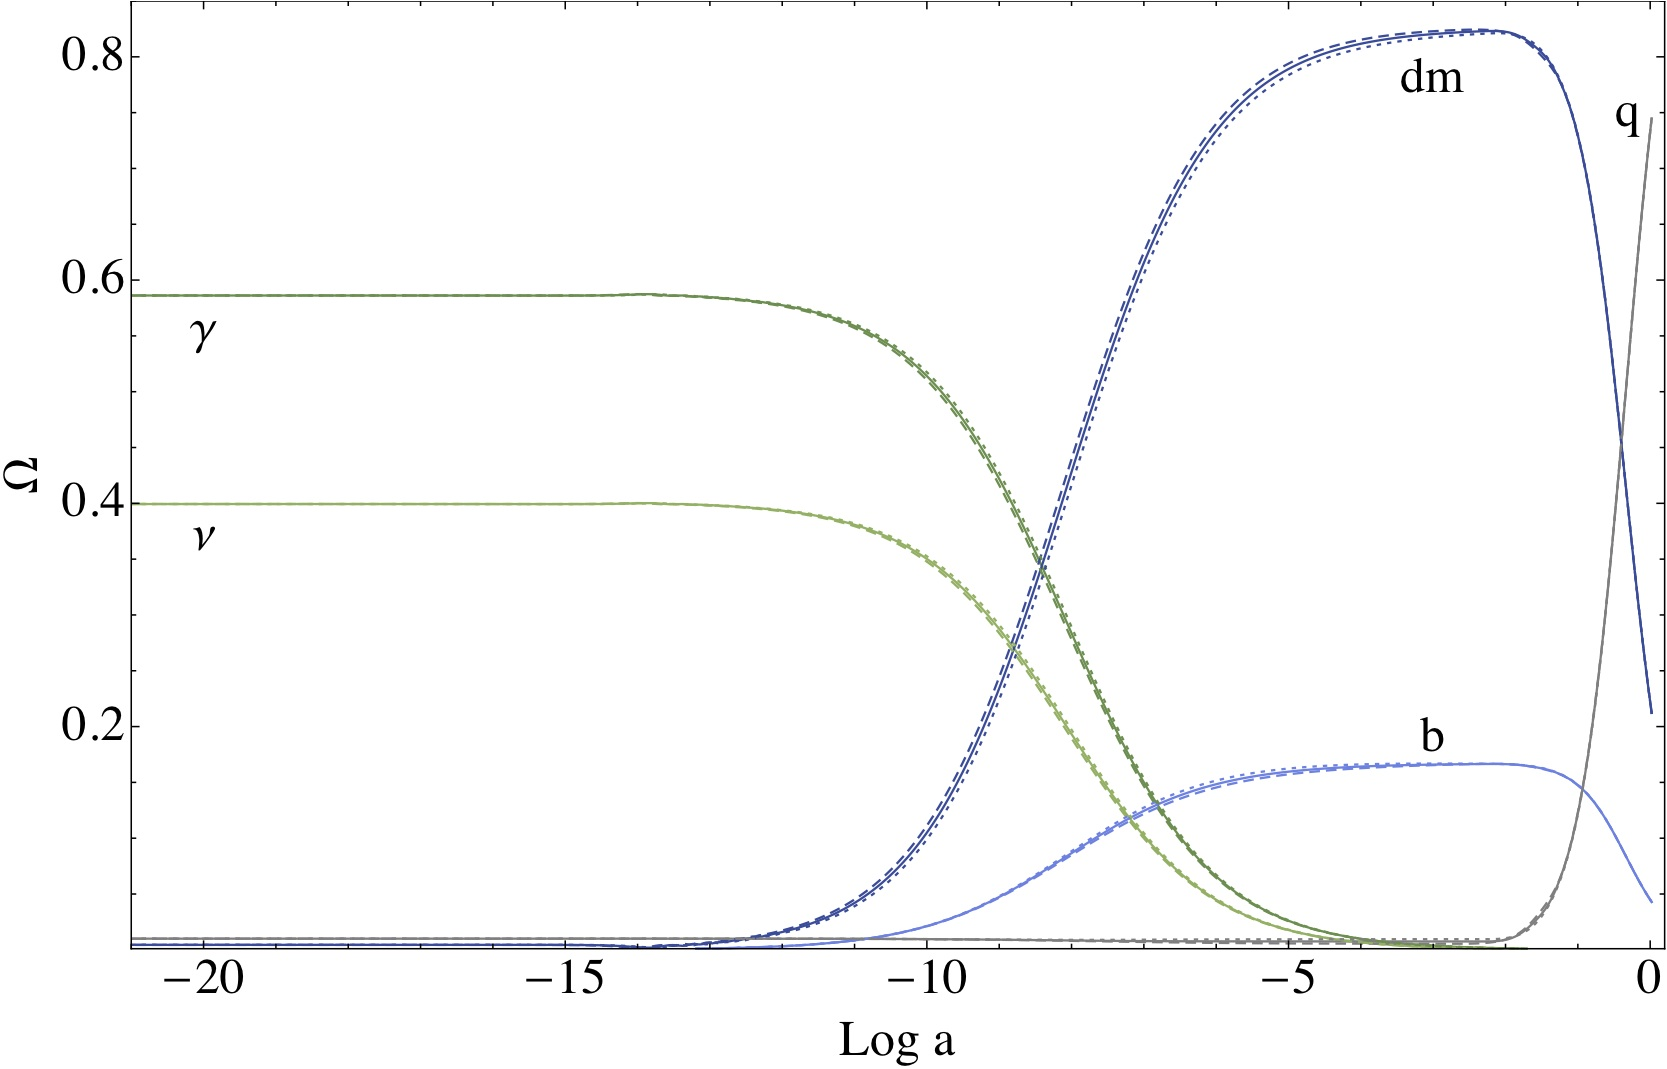
\includegraphics[scale=0.26]{grafica}
\caption{Gr\'afica que muestra la evoluci\'on de los par\'ametros de densidad desde el Big Bang hasta el d\'ia  de hoy. Aqu\'i vemos que  $\gamma$ corresponde a los fotones, $v$ a los neutrinos, $dm$ a materia oscura, $b$ a materia bari\'onica y $q$ a energ\'ia oscura.} 
\end{figure}




\section*{Agujeros negros primordiales}
\subsubsection*{?`Qu\'e es un agujero negro?}
Un agujero negro podemos definirlo como una regi\'on en el espacio-tiempo cuya distorci\'on genera una fuerza gravitacional tan fuerte que puede absorber cualquier tipo de part\'icula incluyendo la luz. 
Estos objetos se forman debido al colapso gravitacional de una estrella muy masiva donde las fuerzas nucleares ya no son lo suficientemenete fuertes para impedir que la estrella se contraiga sobre s\'i misma debido a su gravedad, originando una singularidad espacio-temporal.
\subsubsection*{Espacio-tiempo}
Cuando se habla de teor\'ia general de la relatividad normalmente se hace una analog\'ia para comprender mejor la idea del espacio-tiempo. Imaginemos un pedazo de tela extendido, ahora supongamos que dejamos caer una bola de metal de 1 kilogramo, podemos notar 2 cosas inmediatamente. La primera es que el objeto debido a su masa distorciona la tela y si colocamos otros objetos cerca de la bola estos teneder\'an a irse hacia ella. Segundo, la distorci\'on en la tela es proporcional a la masa, lo que significa que mientras m\'as masivo sea el objeto m\'as distoriona la tela.

Esto es exactamente lo que pasa con el espacio-tiempo seg\'un la teor\'ia de Einstein, la tela es el espacio-tiempo, la bola de metal son los objetos astron\'omicos como: planetas, estrellas, etc. Y la distorci\'on representa la fuerza que conocemos como gravedad.
En un agujero negro el colapso es tan enorme que se genera un fen\'omeno llamado singulardidad, un punto infinitamente peque\~{n}o y denso en donde se concentra toda la materia que alguna vez pertenecio a la estrella.
Esta singularidad es rodeada por un horizonte de sucesos el cual determina la regi\'on en donde ninguna part\'icula puede escapar debido a que la gravedad se intensifica enormemente dentro de dicha regi\'on.

\subsubsection*{?`Qu\'e es un agujero negro primordial (PBH)?}
Un PBH es en escencia un agujero negro que se form\'o en los primeros instantes del Big Bang debido a la alta densidad y fluctuaciones en el universo temprano, estas fluctuaciones originaron regiones en donde habr\'ia una gran acumulaci\'on de materia la cual eventualmente colapsar\'ia gravitacionalmente originando los PBHs. Recordemos que durante los momentos que siguieron al Big Bang hab\'ia una enorme presi\'on y temperatura estas condiciones extremas junto con una peque\~{n}a perturbaci\'on en la densidad de materia pueden dar paso a un agujero negro.

Si hacemos una comparaci\'on de la densidad cosmol\'ogica en un tiempo t despu\'es del Big Bang con la densidad asociada a un agujero negro de masa M [9], tendremos que la masa de un PBH durante la epoca de radiaci\'on es aproximadamente igual a la masa del horizonte de Hubble y vendr\'a dada por:
\begin{equation}
M_{PBH}(t)\approx M_H=10^{15}*\left(\frac{t}{10^{-23} s}\right)  gramos
\end{equation}
$M_{PBH}$ es la masa del PHB y $M_H$ es la masa del horizonte de Hubble.

Esta ecuaci\'on nos dice que de acuerdo al momento de creaci\'on del agujero negro ser\'a la masa asociada a \'el, por ejemplo: si tenemos un agujero negro que se form\'o en $t=10^{-43} s$ (tiempo de Plack) su masa ser\'a $M=10^{-5} gramos$ y si tenemos un agujero negro que se form\'o en $t=1 s$ entonces $M=10^{5} M_{solar}$ donde $M_{solar}=1.98\times10^{30} kg$. Este amplio espectro de masas (que ser\'a tratado con m\'as detalle en las proximas secciones) es una de las razones por la que los PBHs se propusieron como candidatos a materia oscura.

Un importante detalle es que si un agujero negro se form\'ara en la actualidad su masa debe ser superior a una masa solar.
Si tomamos en cuenta que la masa del horizonte de Hubble al final del periodo de inflaci\'on del universo en terminos de la temperatura de recalentamiento $T_{RH}$ es:
\begin{equation}
M_H=10^{17}g*\left(\frac{10^{7}GeV}{T_{RH}}\right)^{2}
\end{equation}
Podemos darnos una idea de la masa de un PBH y aunque la temperatura de recalentamiento depende del modelo infacionario que se considere, ciertamente la mayor\'ia de los modelos $T_{RH}$ es del orden de $10^{10} GeV$ (ya que leptogenesis no permite valores menores a $10^{9} GeV$).
Esto significa que pudieron formarse PBHs con masas muy peque\~{n}as (alrededor de $10^{11} g$) comparadas con las que se formaron 1 segundo despu\'es del Big Bang. Estas masas tan bajas impulsaron la investigaci\'on sobre las propiedades cu\'anticas de los PBHs [7].

\subsubsection*{Radiaci\'on de Hawking}
Fue hasta 1976 cuando el cient\'ifico Stephen Hawking demostr\'o matem\'aticamente que los agujeros negros pod\'ian emitir radiaci\'on, perder masa y eventualmente evaporarse, lo que iba totalmente en contra de lo que se pensaba de un agujero negro. 
Para entender esto necesitamos conocer lo que son las fluctuaciones cu\'anticas, este fen\'omeno se debe al principio de incertidumbre en su forma de indeterminaci\'on tiempo-energ\'ia cuya expresi\'on matem\'atica es:
\begin{equation}
\Delta{E}*\Delta{\tau}\geq\frac{h}{4\pi}
\end{equation}
Debido a la aparente violaci\'on del principio de conservac\'ion de la energ\'a se introduce un efecto cu\'antico en el que se generan pares de part\'icula y antipart\'icula virtuales durante un lapso de tiempo muy corto provenientes del vac\'io. 
Si estas part\'iculas virtuales se generan en la cercan\'ia del horizonte de eventos de un agujero negro, una de ellas puede ser atrapada por la intensa gravedad (dentro del horizonte) y la otra puede escapar; si la part\'icula logra escapar, la energ\'ia de dicho proceso ser\'a proveniente del agujero negro. Lo que significa que el agujero negro deber\'a perder energ\'ia para compensar la creaci\'on de las part\'iculas que separ\'o. Est\'e fen\'omeno se denomina radiaci\'on de Hawking ya que el agujero negro por consecuencia emite radiaci\'on y a su vez la masa dismunuye.
La radiaci\'on de Hawking para un agujero negro est\'atico es
\begin{equation}
T=\frac{\hbar c^{3}}{8 \pi G M k}=10^{-7} \left(\frac{M}{M_{solar}}\right)^{-1} K
\end{equation}
Donde el tiempo de evaporizaci\'on esta dado por 
\begin{equation}
\tau(M)\approx \frac{\hbar c^{4}}{G^{2} M^{3}}=10^{64} \left(\frac{M}{M_{solar}}\right)^{3}
\end{equation}
Lo que nos dice que mientras m\'as peque\~no sea la masa del agujero negro m\'as rapidamente se evaporar\'a, de hecho utilizando las ecuaci\'ones anteriores podemos ver facilemente que solo los agujeros negros que se crearon antes de $10^{-23} s$ cuya masa ser\'a m\'as peque\~na que $10^{15} g$ se evaporar\'an en la actualidad, estos agujeros negros emitar\'an fotones del orden de $100 MeV$ y son los que con el equipo y t\'ecnicas adecuadas podr\'ian ser detectados.

\subsubsection*{Proceso de Formaci\'on de PBHs a partir de inhomogeneidades}
Como ya hemos mencionado los PBHs pudieron haberse formado en los primeros instantes del Big Bang, debido a la alta densidad en el universo. Pero adem\'as necesitamos que haya fluctuaciones para que las regiones en donde haya sobre densidad detengan su expansi\'on y colapsen.
Los primeros c\'alculos realizandos por Bernard Carr y Hawking revelaron que dichas regiones que eventualmente generar\'ian un PBH deb\'ian ser m\'as grande que la longitud de Jeans
\begin{equation}
r_J=4\pi \frac{\sqrt{w}}{5+9w}d_H
\end{equation}
Donde $d_H$ es el horizonte de part\'iculas (que es del orden del radio de Hubble $r_H=1/H$) y $w$ una constante de la ecuaci\'on de estado
\begin{equation}
p=w\rho
\end{equation}
(Con $ 0<w<1$, por ejemplo para la \'epoca de radiaci\'on $w=1/3$).

Pero tambi\'en dicha regi\'on no puede ser m\'as grande que el tama\~no del horizonte ya que de ser as\'i formar\'ia un universo cerrado separado del nuestro.
Veremos 2 implicaciones muy importantes de lo anterior. Primero como hab\'iamos mencionado, para un PBH que se form\'o un tiempo $t$ d\'espues del Big Bang \'este debe ser del orden de la masa del horizonte. 

Y segundo, se requiere que la regi\'on que colapsar\'a en un PBH debe ser m\'as grande que una cierta densidad critica $\delta=\Delta M/M_{H}$. Donde $\delta > w$.

A lo largo de los a\~nos muchos autores han calculado valores para esta densidad critica ya que esta es escencial si queremos calcular el espectro de masas de los PBHs.

El primer c\'alculo fue realizado por Carr en 1975, el cual encontr\'o que $\delta \approx 1/3$. Carr asumi\'o un modelo de Friedmann cerrado con peque\~nas perturbaciones en la densidad dando como resultado un espectro de masas que solo depende de la amplitud cuadr\'atica media $\epsilon$ en la densidad de flutaciones y de la ecuaci\'on de estado (9).
Para la \'epoca de radiaci\'on tomando $w=1/3$ y asumiendo una distribuci\'on gaussiana con simetr\'ia esf\'erica para la densidad de fluctuaciones, la fracci\'on de regiones de masa $M$ que colapsar\'an es[9]:

\begin{equation}
\beta(M)\sim \epsilon(M)*exp\left(\frac{-\gamma^2}{2\epsilon(M)^2}\right)
\end{equation}

Donde $\epsilon(M)$ es la amplitud de fluctuacion con una masa horizonte M.
Uno de los puntos m\'as importantes a resaltar de los c\'alculos realizados por Carr es que los PBHs s\'olo pueden tener un espectro de masas amplio si las fluctuaciones son invariantes escalares. Si \'este es el caso el espectro de masas es:
\begin{equation}
\frac{dn}{dM} = (\alpha -2)(M/M_*)^{-\alpha} M_* ^{-2} \Omega_{PHB} \rho_{critica} 
\end{equation}

Donde $M_*\approx 10^{15} g$, $\Omega_{PBH}$ es el par\'ametro de densidad total de los PBHs y $\alpha$ est\'a dada por:

\begin{equation}
\alpha=\left(\frac{1+3w}{1+w}\right) + 1
\end{equation}

(Si $w=1/3$ entonces $\alpha=5/2$, esto significa que si la densidad de los PBHs es m\'as grande que $M$ decaen como $M^{-1/2}$, entonces la mayor parte de esta densidad est\'a contenida en los PBHs m\'as peque\~nos).

Por \'ultimo el par\'ametro de densidad actual $\Omega_{PBH}$ asociado a un PBH en un tiempo $t$ esta relacionado con $\beta$ por:

\begin{equation}
\Omega_{PBH}=\beta \Omega_R (1+z) \approx 10^{18} \beta \left(\frac{M}{10^{15}}\right)^{-1/2}
\end{equation}

Donde $M$ es la masa de la regi\'on colapsada, $z$ el corrimiento hacia el rojo y $\Omega_R$ es el par\'ametro de densidad del fondo de microondas ($\Omega_R \approx 10^{-4}$). 

Los c\'alculos realizados por Carr dan soporte al ampio espectro de masas que podr\'ian tener los PBHs y con esto muchos cient\'ificos han propuesto modelos que mejoran la teor\'ia de Carr para poder observarlos.

\subsubsection*{Observaciones de PBHs}
Con la reciente detecci\'on de ondas gravitacionales se ampliaron los m\'etodos de detecci\'on de objetos masivos como agujeros negros y PBHs y se han propuesto algunos nuevos.

LIGO y VIRGO lograron detectar ondas gravitacionales de sistemas binarios de agujeros negros, y existe la posibilidad de que estos agujeros negros sean primordiales debido a que, al menos en teor\'ia, las masas en los modelos can\'onicos sobre la distribuci\'on de materia oscura est\'an dentro del rango especificado por LIGO. No es seguro que el sistema binario de agujeros negros est\'e formado de PBHs, pero no podemos descartar la opci\'on de que as\'i sea. 

Hay propuestas de utilizar un m\'etodo llamado ``microlente difractivo'', que consiste en realizar observaciones de microlente gravitacional en qu\'asares usando PBHs sub-lunares como lentes. \'Este m\'etodo es reciente y a\'un no est\'a del todo implementado pero, si funciona, podr\'ia usarse para determinar el porcentaje de materia oscura que est\'a hecho de PBHs, pues es posible que la materia oscura est\'e formada de otros componentes distintos.



\section*{Conclusiones}

Los PBHs cumplen con las propiedades que se espera tenga la materia oscura, como su poca o nula interacci\'on con la luz, su gran densidad y su aparente distribuci\'on en la galaxia, pero esto no es mas que un modelo propuesto, dado que a\'un no se ha logrado demostrar que existen los PBHs directamente, y las observaciones encuentran objetos que podr\'ian ser PBHs, pero no se sabe con seguridad si lo son o no, por lo que tal vez sea necesario esperar a experimentos m\'as sensibles de detecci\'on de ondas gravitacionales, como el telescopio Einstein, DECIGO (Deci-Hertz Interferometer Gravitational wave Observatory) y BBO (Big Bang Observer).

\subsection*{Bibliograf\'ia}
\textbf{}
\\.[1]Blais, D., Kiefer, C. and Polarski, D. (2002). Can primordial black holes be a significant part of dark matter?. Physics Letters B, 535(1-4), pp.11-16.
\\.[2]Inomata, K., Kawasaki, M., Mukaida, K., Tada, Y. and Yanagida, T. (2017). Inflationary primordial black holes as all dark matter. Physical Review D, 96(4).
\\.[3]Lacki, B. and Beacom, J. (2010). PRIMORDIAL BLACK HOLES AS DARK MATTER: ALMOST ALL OR ALMOST NOTHING. The Astrophysical Journal, 720(1), pp.L67-L71.
\\.[4]Frampton, P., Kawasaki, M., Takahashi, F. and Yanagida, T. (2010). Primordial black holes as all dark matter. Journal of Cosmology and Astroparticle Physics, 2010(04), pp.023-023.
\\.[5]Hawkins, M. (2011). The case for primordial black holes as dark matter. Monthly Notices of the Royal Astronomical Society, 415(3), pp.2744-2757.
\\.[6]Carr, B., Kühnel, F. and Sandstad, M. (2016). Primordial black holes as dark matter. Physical Review D, 94(8).
\\.[7]Hidalgo Cuellar, J. (2009). Primordial black holes in non-linear perturbation theory. Doctorado. University of London.
\\.[8]Kohri, K. and Yokoyama, J. (1999). Primordial black holes and primordial nucleosynthesis: Effects of hadron injection from low mass holes. Physical Review D, 61(2).
\\.[9]B. J., C. (2005). Primordial Black Holes: Do They Exist and Are They Useful?. Inflating Horizon of Particle Astrophysics and Cosmology.
\\.[10]Planck Collaboration (2015). Planck 2015 results. XIII. Cosmological parameters. arXiv:1502.01589 [astro-ph.CO]
\\.[11]T. Naderi, A. Mehrabi, S. Rahvar1. (2016). Primordial black hole detection through diffractive microlensing. arXiv:1711.06312
\\.[12]Hawkins, M. (2011). The case for primordial black holes as dark matter. arXiv:1106.3875
\\.[13]Beyer, J. (2014). Linear Perturbations in coupled cosmon-bolon cosmology. arXiv:1407.0497
\\.[14]The Virgo collaboration (2017). Gravitational waves from a binary black hole merger observed by LIGO and Virgo. https://www.ligo.caltech.edu/news/ligo20170927


\end{document}
